\documentclass{thesisbeamer}

\usepackage{caption}
\usepackage{comment}
\usepackage{amsmath}
\usepackage{bm}
\usepackage{multicol}
\usepackage{xcolor}
\usepackage{tabularx}
\usepackage{optidef}
\usepackage{mathtools}

\usepackage{comment}
\usepackage{graphicx}
\usepackage{subcaption}
\captionsetup{compatibility=false}

\title[Making Flips with Quadrotors in Constrained Environments]{Making Flips with Quadrotors in Constrained Environments}
\author[Elie Hatem]{Elie Hatem \newline ~ \newline \normalsize{Advisors: Dr. Sebastien Briot, Dr. Isabelle Fantoni}}
\date{\today}

\setbeamerfont{caption}{size=\tiny}

\newcommand\Fontvi{\fontsize{9}{10}\selectfont}


\bibliography{../biblio}

% video will work on Linux (with Okular) or OS X, for other OS's or viewers find your own way to do it
%\videoOSX	% for OS X 
\videoOFF

\AtBeginSection[]
{
     \begin{frame}[allowframebreaks]
         \frametitle{Table of Contents}
         \tableofcontents[currentsection]
     \end{frame}
}

\begin{document}

\MakeTitleNoFoot

% \begin{frame}[allowframebreaks]
% 	\frametitle{Table of Contents}
%     \tableofcontents
% \end{frame}


\section{Introduction}

\begin{frame}
\frametitle{The Quatrotor Platform}
\Fontvi

\begin{figure}[t]
     \centering
     \begin{subfigure}[b]{0.45\textwidth}
         \centering
         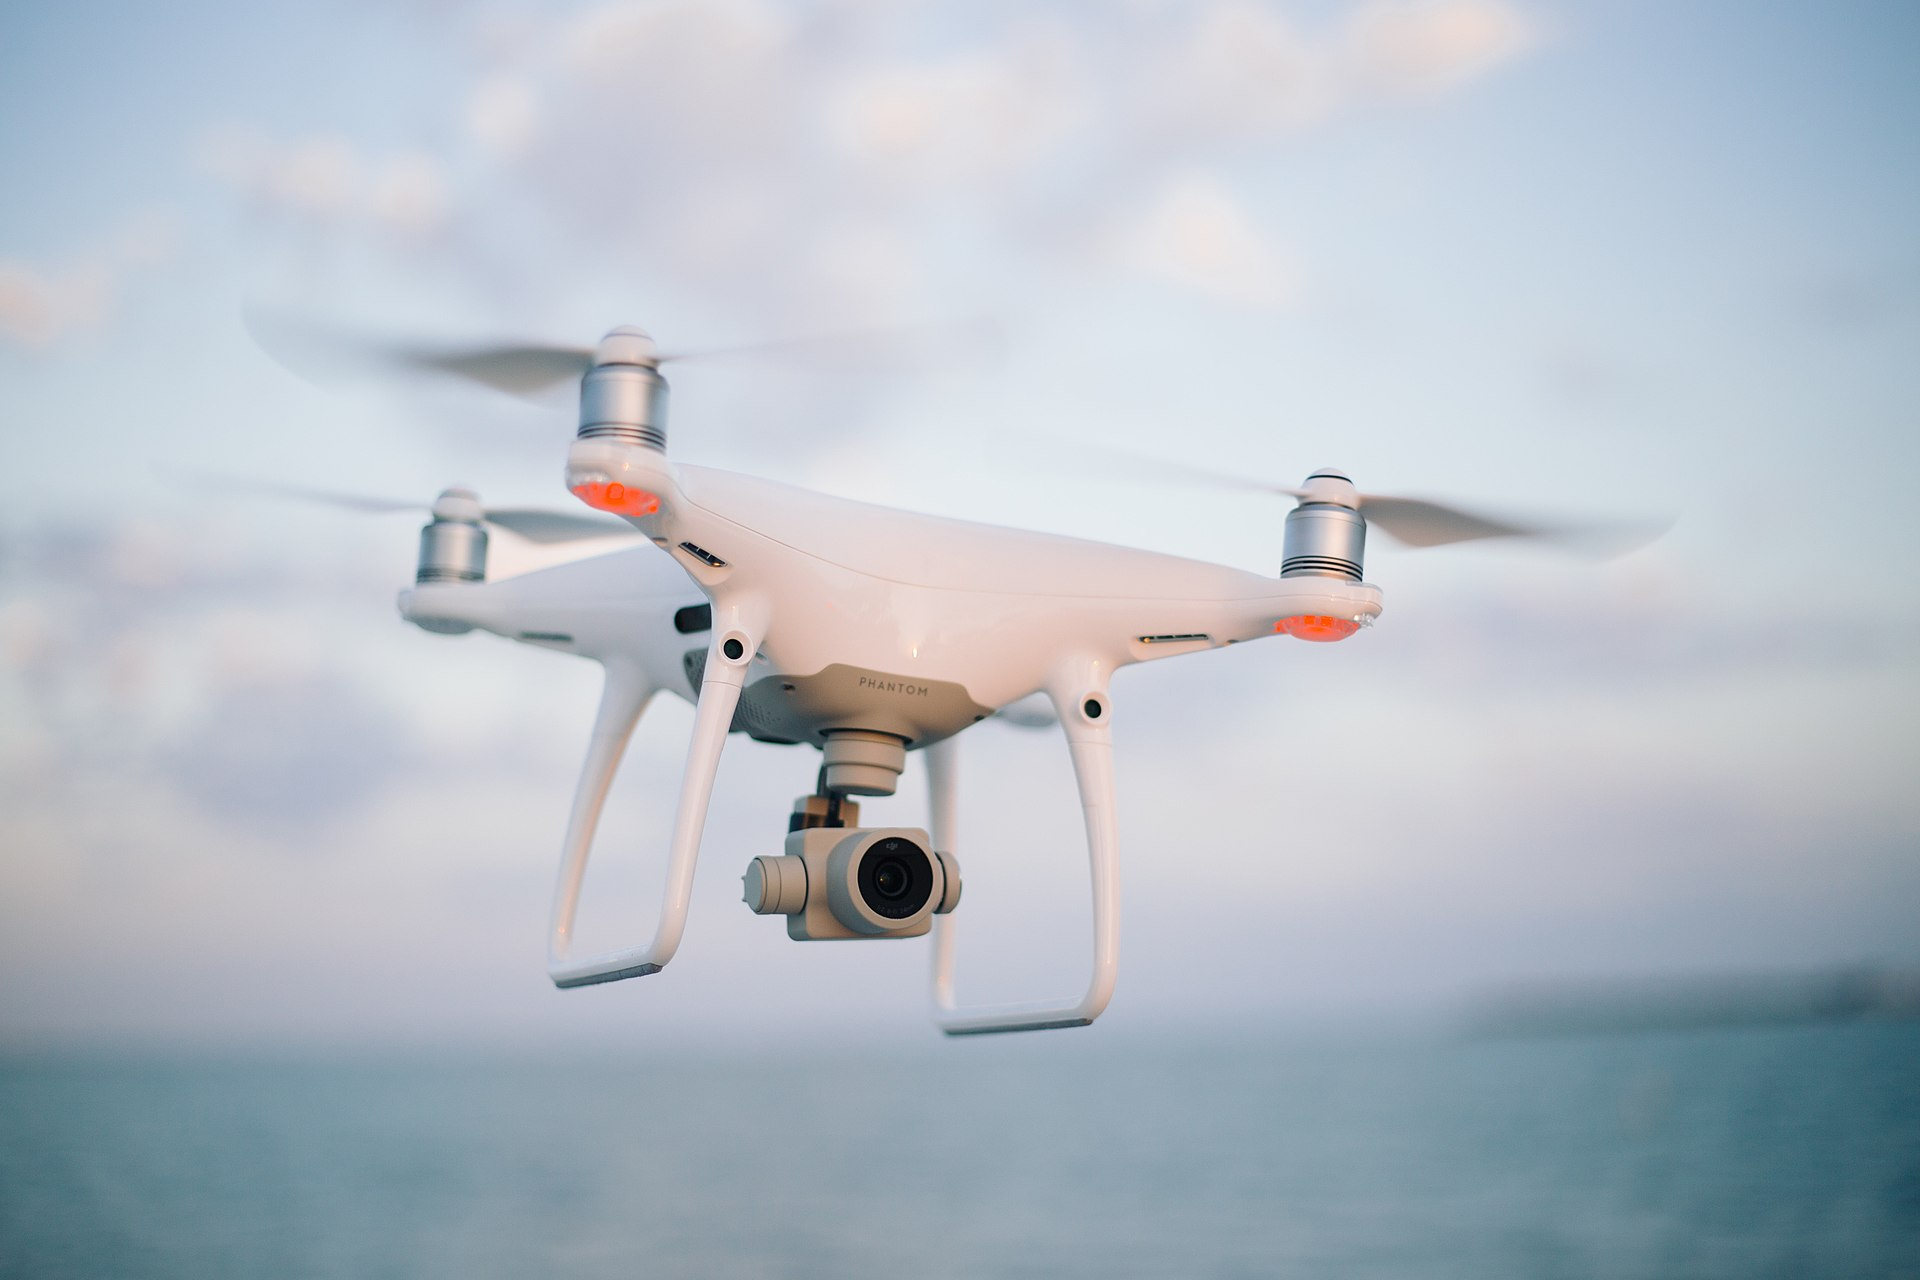
\includegraphics[width=\textwidth]{Images/Introduction/drone}
         \caption[Caption for LOF]{DJI Phantom quadcopter (UAV)\protect\footnotemark}
         \label{fig:drone}
     \end{subfigure}
     \hfill
     \begin{subfigure}[b]{0.45\textwidth}
         \centering
         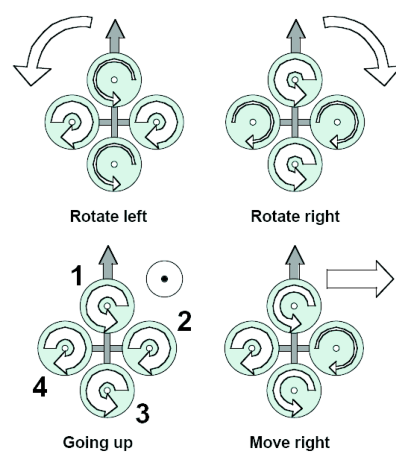
\includegraphics[width=0.6\textwidth]{Images/Introduction/propeller_direction.svg}
         \caption{Quadrotor Concept. Width of the arrows is proportional to the angular speed of the propellers\protect\footnotemark}
         \label{fig:propeller_directions}
     \end{subfigure}
        \caption{Commercial quadrtotor platform (left) and quadrotor concept (right).}
        \label{fig:three graphs}
\end{figure}

\footnotetext[1]{\tiny{\url{https://en.wikipedia.org/wiki/Quadcopter\#/media/File:Quadcopter_camera_drone_in_flight.jpg}}}
\footnotetext[2]{\tiny{Design and control of quadrotors with application to autonomous flying, 2007, S. Bouabdallah}}

\end{frame}


\begin{frame}
\frametitle{The Quatrotor Platform}
\Fontvi

Over the last few years, quadrotors have gained large popularity in academia and industry. Because, they are:

\begin{itemize}
	\item Simple to design and assemble using relatively cheap components.
	\item Different use cases: aerial photography, agriculture, surveillance tasks, etc.
	\item Quite agile and maneuverable during flight, especially when compared to other types of UAVs.
\end{itemize}

\end{frame}

\begin{frame}
\frametitle{Main Challenges}

\begin{block}{One of the main challenges}
	Capability to design control and planning methods to allow tracking aggressive trajectories.
\end{block}

This is due to: 
\begin{itemize}
	\item The fast dynamics associated with the small dimensions of such agile quadrotors.
	\item Several dynamic effects that will become important during aggressive flight maneuvers.
	\item The motors will be commanded high speeds and accelerations, which will cause them to saturate and introduce delays.
\end{itemize}


\end{frame}



\begin{frame}
\frametitle{Goals of the Master Thesis}
\Fontvi

The goals of the master thesis: 

\begin{itemize} % [<+->]
	\item Study of multi-flip maneuvers.
	\item Implement Model Predictive Control to solve the presented issues.
	\item Perform the maneuvers in a constrained environment.
\end{itemize}

\begin{figure}[h]
     \centering
     \begin{subfigure}[h]{0.4\textwidth}
         \centering
         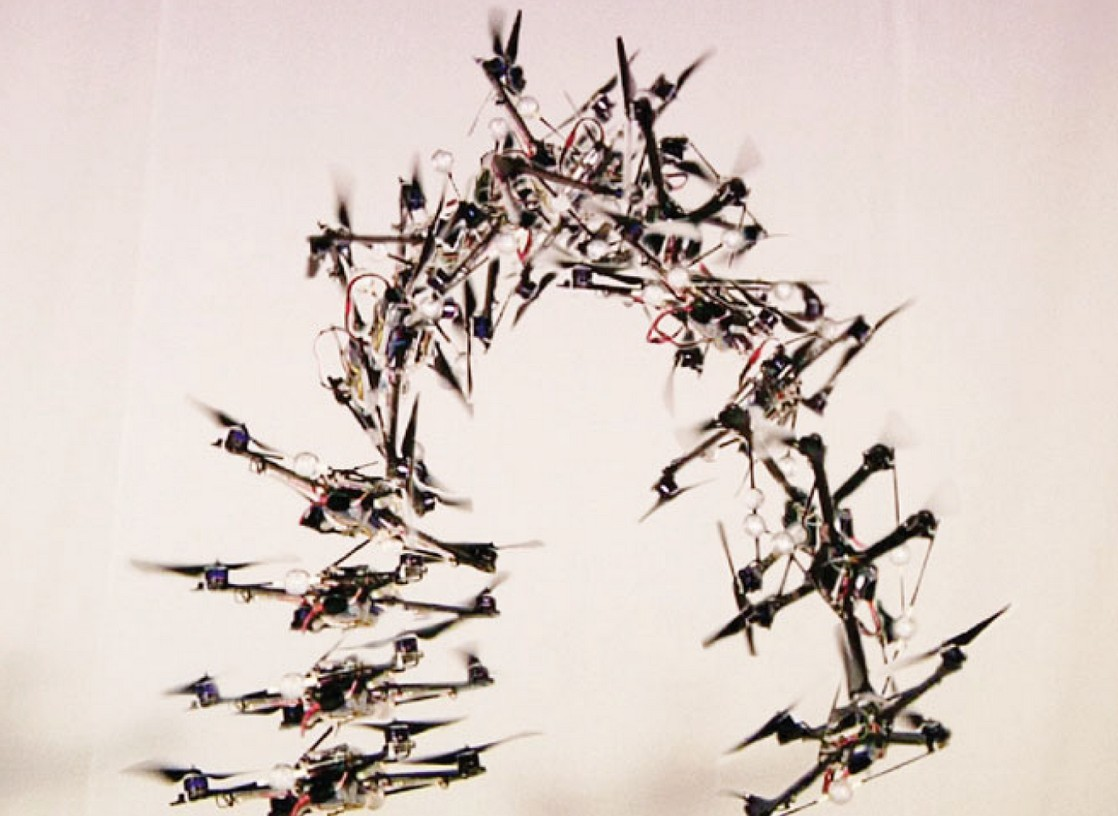
\includegraphics[width=0.9\textwidth]{Images/Introduction/flip}
    \caption{Quadrotor performing a triple flip\protect\footnotemark}
         \label{triple_flip}
     \end{subfigure}
     \hfill
     \begin{subfigure}[h]{0.38\textwidth}
         \centering
         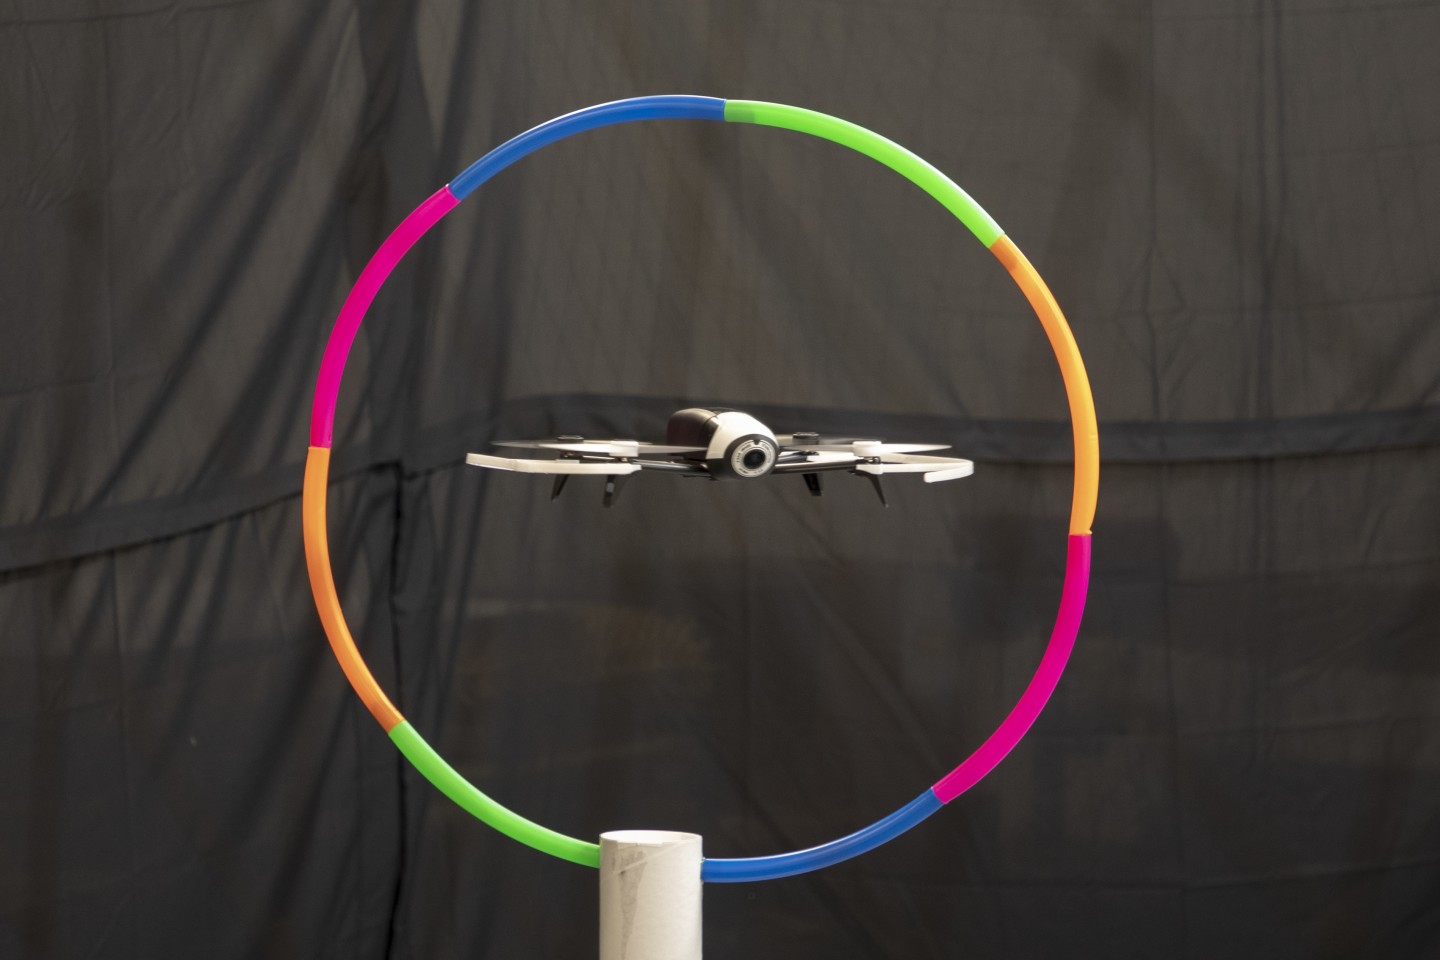
\includegraphics[width=\textwidth]{Images/Introduction/constrained_environment}
         \caption[Caption for LOF]{Quadrotor going though a loop\protect\footnotemark}
         \label{drone_hulahoop}
     \end{subfigure}
        \caption{\tiny{Representation of the issues to be tackled in this master thesis.}}
        \label{fig:three graphs}
\end{figure}

\footnotetext[3]{\tiny{Adaptive fast open-loop maneuvers for quadrocopters, 2012, S. Lupashin and R. D’Andrea}}
\footnotetext[4]{\tiny{ \url{https://newatlas.com/drones/muscle-signals-drone-control/} }}

\end{frame}

\begin{frame}
\frametitle{General Control Architecture of a Quadrotor}

	\Fontvi	
		
	\begin{figure}
		\centering
		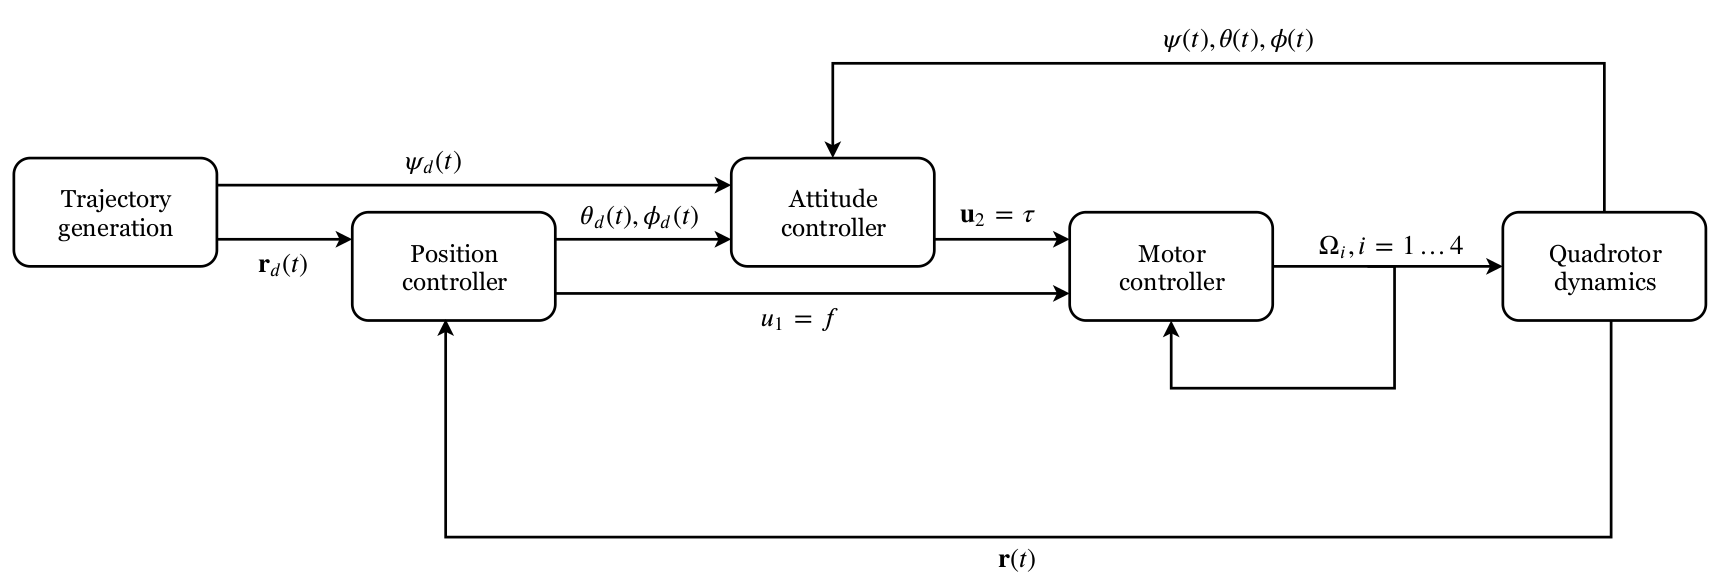
\includegraphics[width=0.9\textwidth]{diagrams/general_control_architecture.png}
		\caption{Diagram of the general control architecture of a quadrotor.}
	\end{figure}
	\begin{itemize} % [<+->]
		\item Position controller: slow rise time - drives translational dynamics errors to 0.
		\item Attitude controller: faster rise time - drives rotational dynamics errors to 0.
		\item Motor controller: fastest rise time - maps the control inputs to motor speeds.
	\end{itemize}
	\begingroup
    \fontsize{9pt}{10pt}\selectfont
    \begin{alertblock}{Remark}
		\begin{itemize}
			\item The designed controller cannot be faster than the one at a lower level.
				\begin{itemize}
					\item \fontsize{9pt}{10pt}\selectfont The orientation cannot be controlled any faster than the motors can be controlled.
				\end{itemize}
		\end{itemize}
		\end{alertblock}
\endgroup						
\end{frame}



\begin{frame}
	\frametitle{Differential Flatness}
	\Fontvi	

	A well-established finding is that the dynamic model of a quadrotor is differentially flat:
	\begin{itemize}
		\item The system with state $\bm{x} \in \mathbb{R}^n$ and input $\bm{u} \in \mathbb{R}^m$ has flat outputs $\bm{y} \in \mathbb{R}^m$ which have the following form:
	
	\begin{equation}
 \textbf{y} = \textbf{y}(\textbf{x}, \textbf{u}, \dot{\textbf{u}},...,\textbf{u}^{(p)})
 \end{equation}

 With, 
 
 \begin{equation}
 	\begin{cases}
 		\textbf{\textsc{x}} = \textbf{x}(\textbf{y}, \dot{\textbf{y}},...,\textbf{y}^{(q)}) \\
 	\\
 		\textbf{u} = \textbf{u}(\textbf{y}, \dot{\textbf{y}},...,\textbf{y}^{(r)}) \\
 	\end{cases}
 \end{equation}	
	
	
	 \item Very useful property in under-actuated systems where $m<n$, such as quadrotors.
	 \item Allows to generate trajectories in the lower dimensional space $m$.
	 \item The trajectories can then be mapped into the full dimensional space $n$.
	\end{itemize}

\end{frame}


\begin{frame}
	\frametitle{Differential Flatness}
	\Fontvi
	
	The standard choice of flat outputs for the quadrotor are:

\begin{equation}\label{flat_outputs}
\textbf{y} = \begin{bmatrix}
x && y && z && \psi \\
\end{bmatrix}^{\intercal}
\end{equation}

As a result:
\begin{itemize}
	\item Trajectories can be designed in the 4-dimensional space.
	\item They can then be mapped to the 6-dimenstional space.
	\begin{itemize}
		\item Since the rotational and translational dynamics are tightly coupled.
	\end{itemize}			
\end{itemize}

\end{frame}

\section{Model Predictive Control}

\begin{frame}
	\frametitle{Model Predictive Control}
	\Fontvi	

	General idea of MPC:
 	\begin{figure}[t]
 		\centering
 		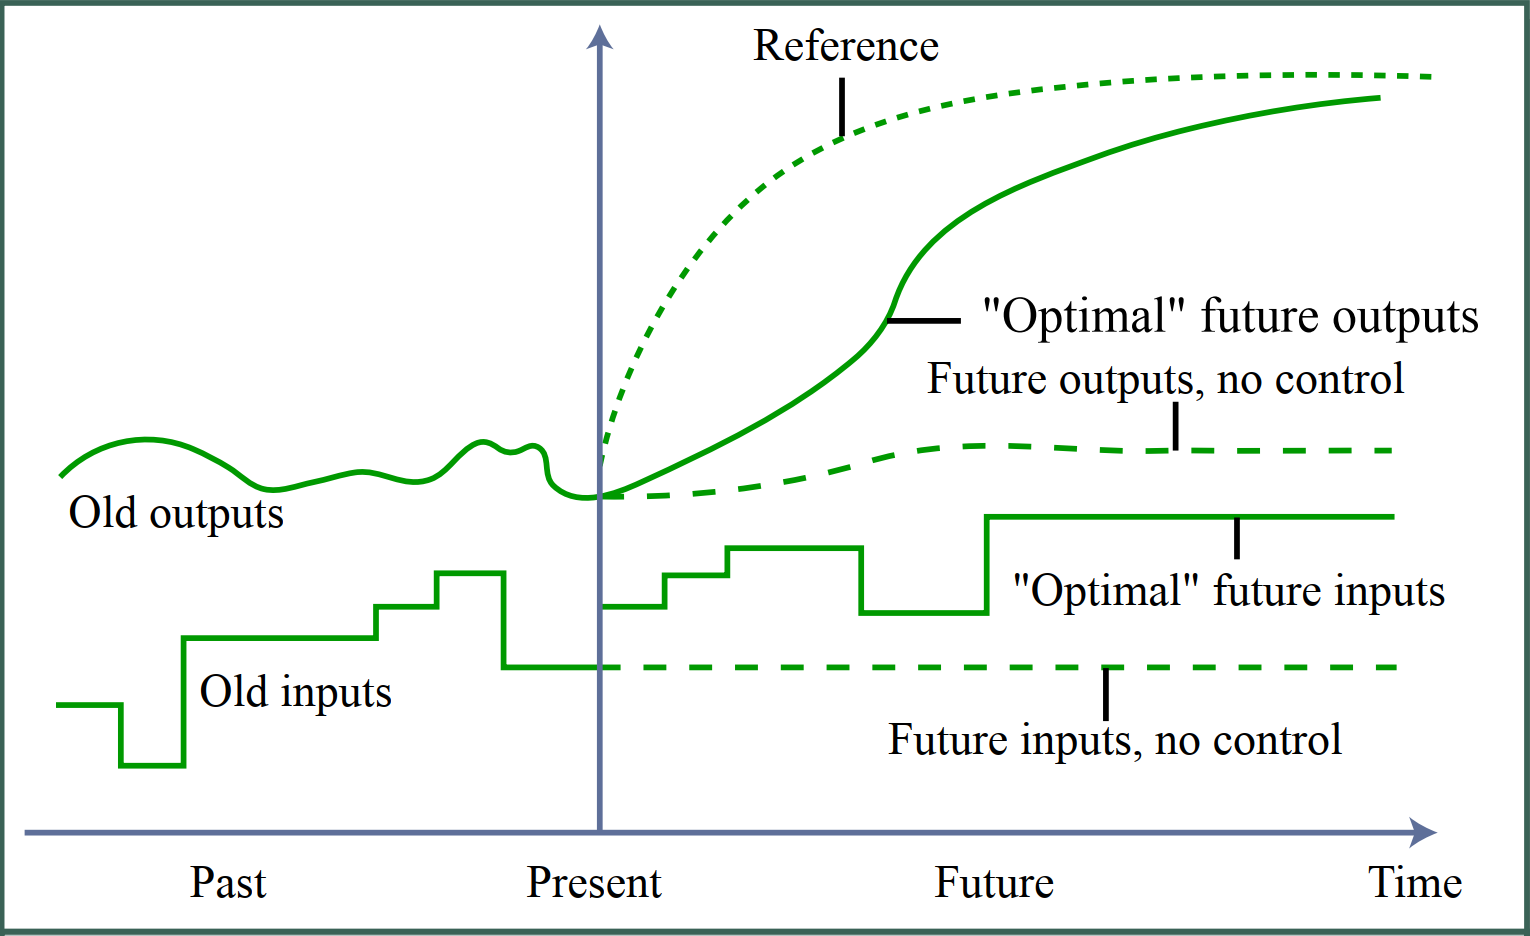
\includegraphics[width=0.5\textwidth]{Images/Control/MPC_general_idea.png}
 		\caption{Basic idea of MPC\protect\footnotemark}
 		\label{MPC_basic_idea}
	\end{figure}  

	\begin{itemize} % [<+->]
		\item It is a \textbf{feedback control} algorithm.
		\item It uses a model to \textbf{predict} future outputs.
		\item It \textbf{solves an online optimization problem} to select the optimal control.
	\end{itemize}

\footnotetext[5]{\tiny{Principles of Optimal Control, 2008, J. How}}

\end{frame}


\begin{frame}
\frametitle{Model Predictive Control}
\Fontvi	

\begin{columns}
\column {0.5\textwidth}
MPC Design parameters:

\begin{itemize} % [<+->]
	\item Sample time.
	\item Prediction horizon.
	\item Control horizon.
	\item Constraints.
	\item Weights.
\end{itemize}\pause


\column {0.5\textwidth}
Choosing proper values for these parameters is important as they affect: 
\begin{itemize}
	\item The controller performance.
	\item The computational complexity of the MPC algorithm.
\end{itemize} 
\end{columns}

\end{frame}



\begin{frame}{MPC applied on quadrotors}
\Fontvi

The most popular uses for MPC in quadrotors are:

\begin{itemize} % [<+->]
	\item Centralized MPC: Single control loop for the system.
	\item Non-centralized MPC: Cascaded control consisting of more than 1 control loop. Examples:
		\begin{itemize}
			\item MPC$_{master}$-MPC$_{slave}$
			\item MPC-PD-P
			\item Other options can be used for the inner loop.
		\end{itemize}
\end{itemize}

\begin{block}{Remark}
\begin{itemize}
	\item Centralized MPC: More accurate, high computation cost.
	\item Non-centralized MPC: Less accurate, lower computation cost. 
\end{itemize}
\end{block}

\end{frame}


\begin{frame}{Centralized MPC}
	\Fontvi

	\begin{columns}
		\begin{column}{0.5\textwidth}
			\begin{figure}
				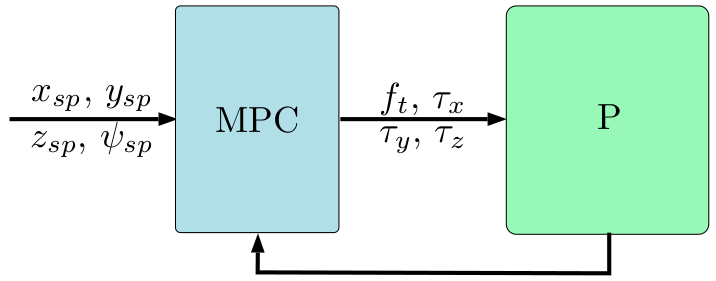
\includegraphics[width=\textwidth]{Images/Control/centralized_mpc.png}
				\caption{Centralized MPC}
			\end{figure}
		\end{column}
		\begin{column}{0.5\textwidth}
			Inputs of centralized MPC:
			\begin{itemize}
				\item Desired $x$, $y$ and $z$ positions and the yaw angle $\psi$.
			\end{itemize}
			Outputs of centralized MPC:
			\begin{itemize}
				\item Total thrust $f_t$.
				\item Torques: $\tau_x$, $\tau_y$ and $\tau_z$
			\end{itemize}
		\end{column}
	\end{columns}
	\vspace{1cm}
	Another version of the centralized MPC exists with:
	\begin{itemize}
		\item Added $\phi$ and $\theta$ angles as outputs.
	\end{itemize}
\end{frame}

\begin{frame}{Non-centralized MPC}
	\Fontvi

			\begin{figure}
				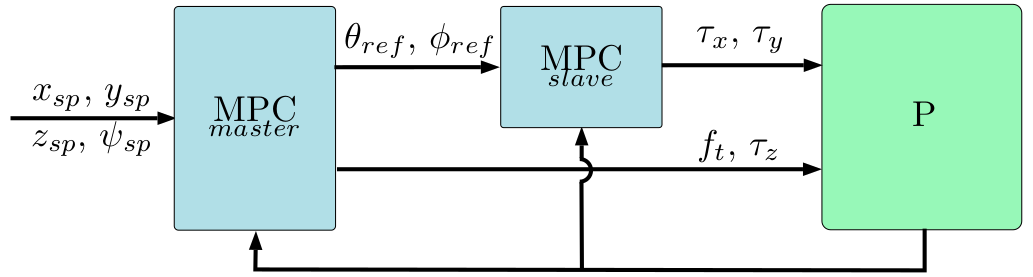
\includegraphics[width=0.7\textwidth]{Images/Control/non-centralized_mpc_1.png}
				\caption{Non-centralized MPC (MPC$_{master}$-MPC$_{slave}$)}
			\end{figure}

			Outer-loop: master MPC
			\begin{itemize}
				\item Inputs: Desired $x$, $y$, $z$, $\psi$.
				\item Outputs: $f_t$, $\tau_z$, $\theta_{ref}$, $\phi_{ref}$.
			\end{itemize}
			Inner-loop: slave MPC
			\begin{itemize}
				\item Inputs: $\theta_{ref}$, $\phi_{ref}$. 
				\item Outputs: $\tau_x$, $\tau_y$.
			\end{itemize}

\end{frame}

\begin{frame}{Non-centralized MPC}
	\Fontvi
	
			\begin{figure}
				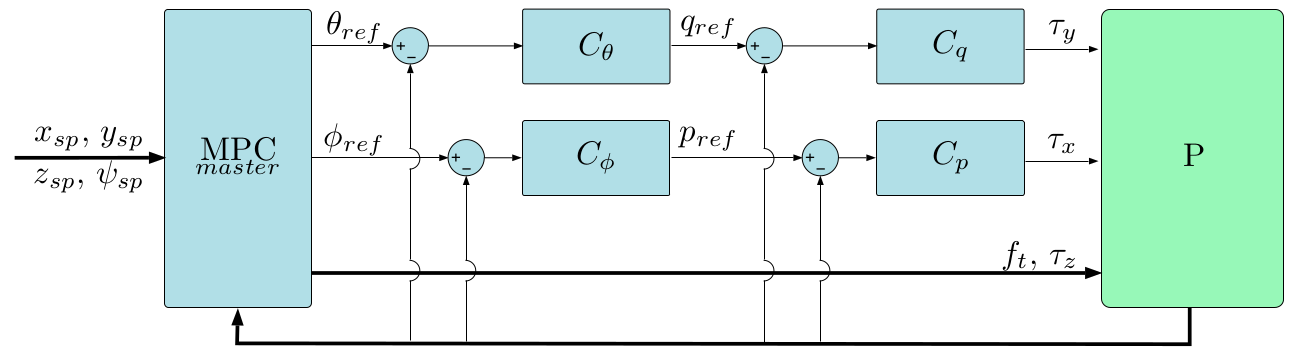
\includegraphics[width=0.7\textwidth]{Images/Control/non-centralized_mpc_2.png}
				\caption{Non-centralized MPC (MPC-PD-P)}
			\end{figure}
			Outer-loop: master MPC
			\begin{itemize}
				\item Inputs: Desired $x$, $y$, $z$, $\psi$.
				\item Outputs: $f_t$, $\tau_z$, $\theta_{ref}$, $\phi_{ref}$ 
			\end{itemize}
			Inner-loop: PD-P controller
			\begin{itemize}
				\item Inputs: $\theta_{ref}$, $\phi_{ref}$. 
				\item Outputs: $\tau_x$, $\tau_y$.
			\end{itemize}
\end{frame}

\begin{frame}[t]{Non-centralized MPC}
	\Fontvi
	Another example of a non-centralized MPC:
	\begin{figure}
		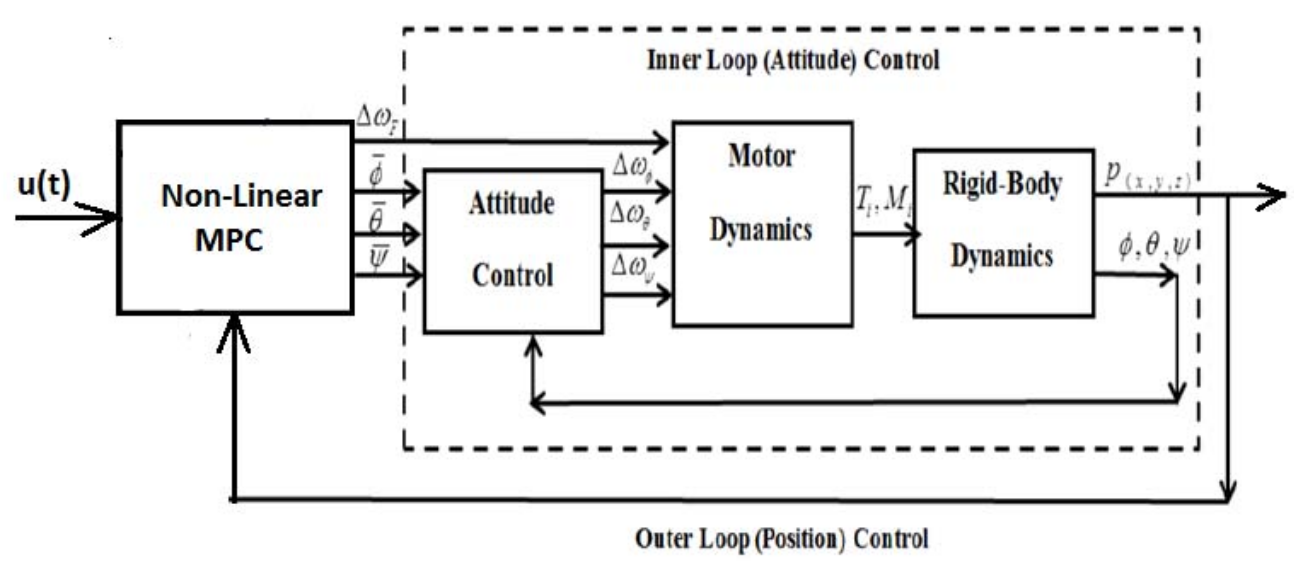
\includegraphics[width=0.7\textwidth]{Images/Control/non-centralized_mpc_3.png}
				\caption{Non-centralized MPC}
	\end{figure}
	\begin{alertblock}{Remark}
	 	The inner-loop can remain fixed, while the outer loop can be reprogrammed to meet the required task.
	 \end{alertblock} 
	 \vspace{5mm}
\end{frame}

\section{acados}

\begin{frame}
	\frametitle{acados}
	\Fontvi
	The software used for implementing MPC controller is \texttt{acados}:
	
	\begin{itemize}
	\item Contains efficient optimal control algorithms implemented in C.
	\item Has a modular architecture enabling rapid prototyping of solution algorithms.
	\item Interfaces to \texttt{C++}, \texttt{Python} and \texttt{MATLAB}.
	\item Uses the high-performance linear algebra package \texttt{BLASFEO}.
	\item Compatible with \texttt{CasADi} expressions.
	\item Deployable on a variety of embedded devices.
	\item Free and open-source software.
\end{itemize}

Main drawback:

\begin{itemize}
	\item Prediction horizon and control horizon must be of same length. 
		\begin{itemize}
			\item This issue can be solved using the real-time iteration (RTI) method.
		\end{itemize}
\end{itemize}

\end{frame}

\begin{frame}
	\frametitle{General Form of the Resulting Nonlinear Program}
	\Fontvi
	
	The general form of the nonlinear program that can be handled by \texttt{acados} is:

    \begin{equation}\label{NLP}
        \begin{aligned}
        \min_{\substack{x_0,\ldots,x_N\\ u_0,\ldots, u_{N-1} \\ z_0,\ldots, z_{N-1}\\  s_0, \ldots, s_N}} \quad & \sum_{k=0}^{N-1}{l_k(x_k, u_k, z_k) + M(x_N) + \sum_{k=0}^N \rho_k(s_k)}\\
        \textrm{s.t.} \quad & \begin{bmatrix}
                                x_{k+1}\\
                                z_k\\
                                \end{bmatrix} = \phi_k(x_k, u_k) \text{ \hspace{2cm}} k=0,1, \ldots, N-1, \\
                            & 0 \geq g_k(x_k, z_k, u_k) - J_{s,k}s_k \text{\hspace{1.25cm}} k=0,1, \ldots, N-1, \\
                            & 0 \geq g_N(x_N) - J_{s,N}s_N, \\
                            & 0 \leq s_k \text{\hspace{3.9cm}} k=0,1, \ldots, N-1
        \end{aligned}
    \end{equation}
    
    And, 
    \begin{equation}
	\rho_k(s_k) = \sum_{i=1}^{n_{s_k}} \alpha_k^i s_k^i + \beta_k^i s_k^{i^2}
\end{equation}

with $\alpha_k^i \in \mathbb{R}, \beta_k^i > 0$.
\end{frame}


\begin{frame}
	\frametitle{Python Interface Overview}
	\Fontvi
		
	\begin{figure}[h]
 		\centering
 		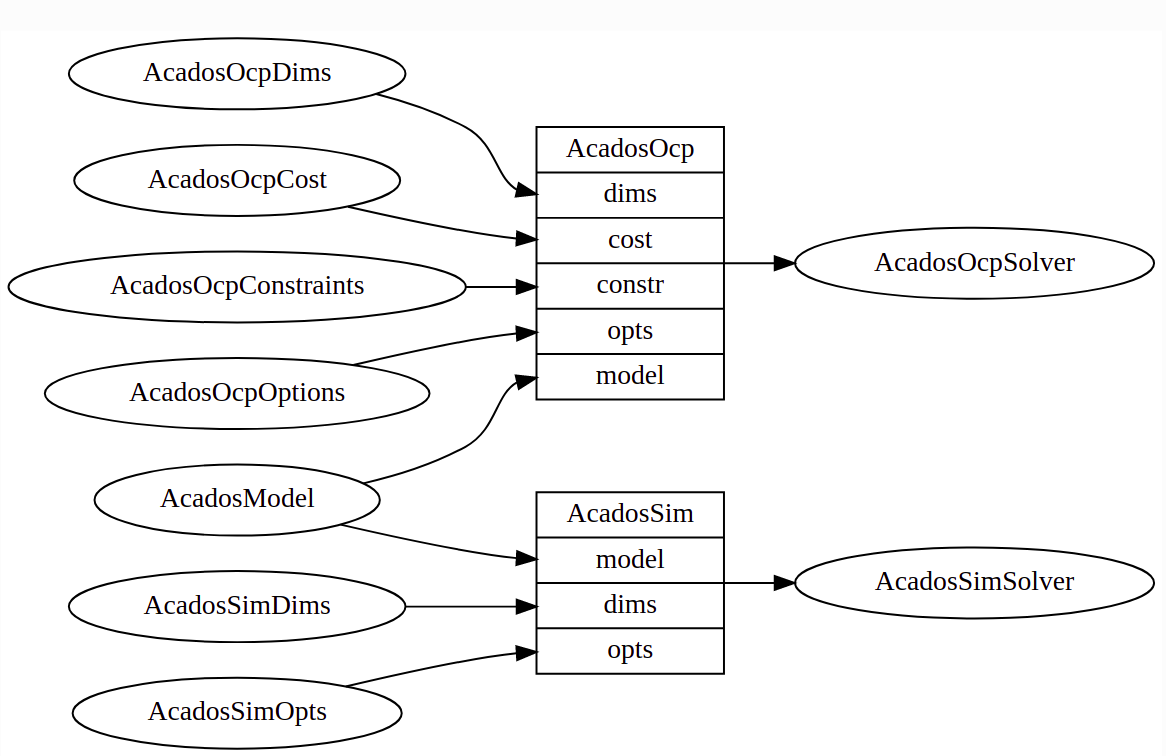
\includegraphics[width=0.8\textwidth]{Images/acados/python_interface.png}
 		\caption{Overview of the Python API classes in acados\protect\footnotemark}
 		\label{fig:python_interface}
 	\end{figure}
 		\footnotetext[6]{\tiny{\url{https://docs.acados.org/python_api/}}}
\end{frame}



















































\begin{frame}{Introduction}
\begin{itemize}[<+->]
\item Some
\item Appearing
\item Bullets
\begin{itemize}
 \item With sub-bullets
\end{itemize}
\end{itemize} 
 \visible<+-> {
 \begin{center}
  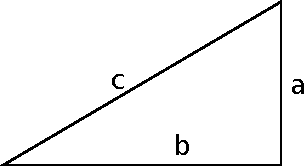
\includegraphics[width=.4\linewidth]{triangle1} \\
  And an appearing figure.
 \end{center}
 }
\end{frame}


\begin{frame}{Main content}
\begin{itemize}[<+>]
\item Some
\item Appearing
  \item And disappearing
\item Bullets
\begin{itemize}[<.>]
 \item With sub-bullets
\end{itemize}
\item That appear and disappear with their parent
\end{itemize}
\end{frame}



\begin{frame}{Main content}
\begin{enumerate}
\item Some	\vfill
\item Numbers
\begin{itemize}
 \item With sub-bullets
\end{itemize}\vfill
\item That appear and the same time\vfill
\item Nicely spaced on the slide
\end{enumerate}
\end{frame}


\begin{frame}{Citations}
 \begin{itemize}[<+->]
  \item Should be done with \textbackslash{fullcite}
  \begin{itemize}[<.->]
   \item \fullcite{pythm001}
  \end{itemize}\vfill
  \item You may also use \textbackslash{smallcite}
  \begin{itemize}[<.->]
   \item \smallcite{pythm001}
   \item It takes less space...
  \end{itemize}\vfill
  \item Check all imported references for:
  \begin{itemize}[<.->]
   \item Name / Journal name / year / editor (journals)
   \item Carefully check conference name (IEEEexplore)
  \end{itemize}
 \end{itemize}
\end{frame}

\begin{frame}{Equations}
\begin{itemize}[<+->]
  \item Have a number if used with \texttt{\textbackslash{begin}\{equation\}}
  \begin{equation}
  \forall \phi: \quad \cos ^2 \phi + \sin^2\phi = 1
  \end{equation}\vfill
  \item Do not have a number if used with \texttt{\textbackslash{begin}\{equation*\}}
    \begin{equation*}
  \forall a, b: \quad (a+b)^2 = a^2 + 2ab + b^2
  \end{equation*}
    \item Another useful environment is simply  \texttt{\textbackslash{begin}\{center\}}
    \begin{center}
    $\forall a, b: \quad (a-b)^2 = a^2 - 2ab + b^2$
    \end{center}
    \begin{itemize}[<+->]
    \item Probably more suited to slides as we use less equation references
  \end{itemize} \vfill\vfill   
  \item Can also be included in the text / bullets
  \begin{itemize}[<+->]
    \item $\forall \phi: \quad  (\cos\phi+\sin\phi)^2 = 2\cos\phi\sin\phi + 1$
  \end{itemize}
\end{itemize}
\end{frame}



\end{document}
